\documentclass[11pt,a4paper]{article}

\usepackage[margin=0.7in]{geometry}

\usepackage[utf8]{inputenc}
\usepackage{graphicx}
\usepackage{microtype}
\usepackage{float}
\usepackage{rotating}
% \usepackage{xcolor}
\usepackage{sectsty}
\usepackage{url}


\usepackage[table,xcdraw]{xcolor}

\usepackage{minted}

\usepackage{hyperref}

\hypersetup{
    colorlinks=true,
    linkcolor=blue,
    filecolor=magenta,      
    urlcolor=blue,
    %urlcolor=cyan,
}

\urlstyle{same}
\definecolor{darkgray}{rgb}{0.66, 0.66, 0.66}
\definecolor{blue(ryb)}{rgb}{0.01, 0.28, 1.0}
\definecolor{dimgray}{rgb}{0.41, 0.41, 0.41}
\sectionfont{\color{cyan}} 
%\sectionfont{\color{blue}} 
%\subsectionfont{\color{cyan}}



\renewcommand{\texttt}[1]{%
  \begingroup
  \ttfamily
  \begingroup\lccode`~=`/\lowercase{\endgroup\def~}{/\discretionary{}{}{}}%
  \begingroup\lccode`~=`[\lowercase{\endgroup\def~}{[\discretionary{}{}{}}%
  \begingroup\lccode`~=`.\lowercase{\endgroup\def~}{.\discretionary{}{}{}}%
  \catcode`/=\active\catcode`[=\active\catcode`.=\active
  \scantokens{#1\noexpand}%
  \endgroup
}

\title{SOEN6461 - Software Design Methodology\\
Design Project\\
Group 9 - Deliverable 3\\
\bigskip
\large{\centerline{\textbf{Professor Yann-Gaël Guéhéneuc}}}
}

\begin{document}

\date{}
\maketitle



% \bigskip
% \bigskip

\begin{table}[H]
\centering
\begin{tabular}{|l|l|}
\hline
\rowcolor[HTML]{FFFC9E} 
\multicolumn{1}{|c|}{\cellcolor[HTML]{FFFC9E}\textbf{Student ID}} & \multicolumn{1}{c|}{\cellcolor[HTML]{FFFC9E}\textbf{Unique email}} \\ \hline
40124288 & plablisenter@outlook.com   \\ \hline
40089008 & user.40089008@gmail.com    \\ \hline
40091878 & SOEN6461cheraghi@gmail.com \\ \hline
40130791 & komal3194p@gmail.com       \\ \hline
\end{tabular}
\end{table}

\vspace{25em}

\centerline{Department of Computer Science and Software Engineering}

\centerline{Gina Cody School of Engineering and Computer Science}

\centerline{Concordia University}

\clearpage

\section{Analysis and Design Requirements}

On one hand, the PADL meta-model allows describing models of (object-oriented) programs.

On the other hand, “PlantUML is a component that allows to quickly write : […] class diagrams” (See \url{https://plantuml.com/}).

Analyze, design, and implement a Visitor that generates a textual description of any PADL model. The description should include \texttt{padl.kernel.IFirstClassEntity} (and possibly all \texttt{padl.kernel.IEntity}) as nodes. The arcs between nodes should describes the different relations between entities (see \texttt{padl.kernel.IRelationship} and its sub-interfaces). The description should conform to the syntax and semantics of \url{https://plantuml.com/classdiagram} so that PlantUML can be called on this description. Demonstrate your implementation by providing textual description of some PADL model as well as the corresponding PlantUML-generated class diagrams.

\section{Implementation}

\subsection{Create PADL meta-model}

The PADL library contains an interface called \texttt{padl.kernel.ICodeLevelModel}. The implementation class of this interface capable of holding the whole PADL meta-model of a set of related classes.

To populate the meta-models, we use the \texttt{create(final ICodeLevelModelCreator aCodeLevelModelCreator)} method, with combination with the \texttt{padl.creator.classfile.CompleteClassFileCreator} class. The source code for creating meta-model is already provided by professor Yann-Gaël Guéhéneuc. We put it inside a singleton class \texttt{plantumlgenerator.utils.MetaModelCreator}. Since the provided source code is just a code snippet, many libraries are required to make it run.

\subsection{Resolve dependencies}

Here is the list of dependencies that are missing/required
\begin{itemize}
    \item package \texttt{padl.kernel} for various interfaces and classes of the meta-model.
    \item package \texttt{padl.analysis} for \texttt{UnsupportedSourceModelException}
    \item package \texttt{padl.creator.classfile} for class \texttt{CompleteClassFileCreator}.
    \item package \texttt{padl.statement.creator.classfiles} for using the class \texttt{ConditionalModelAnnotator} and \texttt{LOCModelAnnotator}
    \item package \texttt{padl.util} for using the class \texttt{ModelStatistics}
\end{itemize}

Each of these packages has a corresponding project in \url{https://github.com/ptidejteam/v5.2} repository. Each project has some dependencies on other libraries as well. To allow separation of each project, we convert each corresponding project into a Maven project and use the Maven package command (\texttt{mvn package}) to create jar files.

Finally, we add all the jar files to \texttt{libs} folder of the main project, then add the dependency in Maven's \texttt{pom.xml} file with \texttt{<scope>} attribute set to \texttt{system}.

The dependency in \texttt{pom.xml} file should look like this and should be repeated with appropriate path for all the required libraries:

\begin{minted}[mathescape,
               linenos,
               numbersep=5pt,
               gobble=2,
               frame=lines,
               framesep=2mm]{xml}
    <dependency>
      <groupId>padl-lib</groupId>
      <artifactId>padl-lib</artifactId>
      <version>5.2</version>
      <scope>system</scope>
      <systemPath>${basedir}/libs/padl.jar</systemPath>
    </dependency>
\end{minted}

For the two packages - \texttt{padl.creator.classfile} and \texttt{padl.statement.creator.classfiles}, we must use the source code (and not jar files) to prevent an exception of type \texttt{java.lang.NoClassDefFoundError} when trying to load a folder of java compiled \texttt{.class} files. This means that the project must be developed using Eclipse IDE. In the future, we will make the project IDE independent using Gradle or Maven.

\subsection{Implement the \texttt{padl.visitor.IGenerator} interface}

We decided to implement the \texttt{padl.visitor.IGenerator} interface for the job, because this interface provides the method \texttt{getCode()}. The \texttt{padl.visitor.IWalker} provides the method \texttt{Object getResult()}, which is really not appropriate for the task we are trying to do.

We created an abstract class \texttt{plantumlgenerator.visitor.PlantUmlVisitor}. The concrete class \texttt{plantumlgenerator.visitor.PlantUmlGenerator} extends this abstract class and implements the \texttt{padl.visitor.IGenerator} interface.

\begin{figure}[H]
\centering
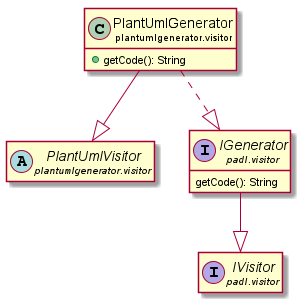
\includegraphics[scale=0.75]{diagrams/implement.png}\color{dimgray}
\caption{The class diagrams of implementation of \texttt{padl.visitor.IGenerator}}
\end{figure}

\subsubsection{Interesting \texttt{open()} and \texttt{close()} methods}

Not all \texttt{open()} and \texttt{close()} methods in \texttt{padl.visitor.IGenerator} were used in the implementation. We only modify the below mentioned \texttt{open()} and \texttt{close()} methods. (All the interfaces used as parameter in open() and close() methods are in \texttt{padl.kernel} package):

\begin{itemize}
    \item open and close for \texttt{IAbstractModel}: \texttt{IAbstractModel} is the root in the hierarchy of PADL meta-model. So, we put the code for  generation of beginning of plantuml code in the open() method, and put the ending code in the close() method.
    \item open and close for \texttt{IPackageDefault} and \texttt{IPackage}: These two interfaces have the same implementation of plantuml code generation. The interface \texttt{IPackageDefault} is for "out of source code" packages (i.e. dependencies package). The \texttt{IPackage} is for normal packages that get compiled.
    \item open and close for \texttt{IGhost}: \texttt{IGhost} is used for classes that have source code in the dependencies libraries (i.e. \texttt{java.io.Serializable})
    \item open and close for \texttt{IClass}: \texttt{IClass} is used for classes that have source code compiled into .class file.
    \item open and close for \texttt{IInterface}: \texttt{IInterface} is used for interfaces that have source code compiled into .class file.
\end{itemize}

\subsubsection{Plantuml code structure and creation}

A typical example of plantuml source code is as follows:

\begin{minted}[frame=lines,framesep=2mm]{text}
@startuml diagram_name

' Packages, classes and interfaces declaration

package packageName {
    class className {
    }
    abstract abstractClassName {
    }
    interface interfaceName{
    }
}

' Classes and interface relationship

className ..|> interfaceName
className --|> abstractClassName

@enduml

\end{minted}

To generate plantuml source code using this template, we use two \texttt{java.lang.StringBuffer} instances. One is for the packages, classes and interface declaration. The other one is for classes and interfaces relationship. The relationship string buffer only appends text in \texttt{open()} methods. Finally, at the \texttt{close(IAbstractModel arg0)} method, we append the relationship string buffer to the declaration string buffer. This kind of implementation allows us to have flexible algorithms to generate code and decouples the responsibilities of each \texttt{StringBuffer} object.

In the end, we return the declaration string buffer using \texttt{toString()} method in \texttt{padl.visitor.IGenerator.getCode()} method.

\subsubsection{An interesting problem (All classes are inherited from \texttt{java.lang.Object}) }

An interesting problem occurred in the generated plantuml code. All java class are extended from \texttt{java.lang.Object} class. This makes the diagram extremely complicated. Therefore, we need to handle the case of classes extending \texttt{java.lang.Object} in the relationship string buffer.

The \texttt{padl.kernel.IClass} interface has \texttt{getName()} method (inherited from \texttt{padl.kernel.IFirstClassEntity}). Comparing the class name with "Object" allows us to distinguish between a normal class and a \texttt{java.lang.Object} class.

\section{How to run the project and coding convention}

\subsection{Coding convention}

The coding conventions can be found here:

\url{https://github.com/huntertran/soen6461-plantuml-generator/wiki/Coding-Conventions}

Since that is a private repository, an exact copy of the document can be found in this public repository:

\url{https://github.com/huntertran/soen6441-riskgame/wiki/Coding-Conventions}

\subsection{How to run the project}

The project must be run from Eclipse IDE.

\begin{itemize}
    \item \textbf{Step 1}: Extract the zip file and import all 3 projects into new Eclipse workspace by select the root folder.
    
\begin{figure}[H]
    \centering
    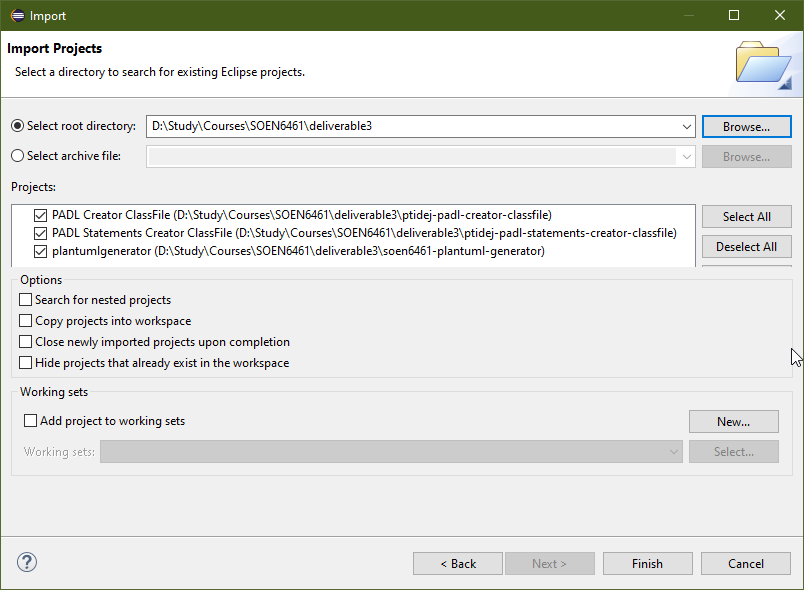
\includegraphics[scale=0.5]{images/open_project.png}\color{dimgray}
    \caption{Import all 3 folder into new eclipse workspace}
\end{figure}
    
    \item \textbf{Step 2}: Select \texttt{plantumlgenerator}. Choose Run / Run As / Java Application.
    
\begin{figure}[H]
    \centering
    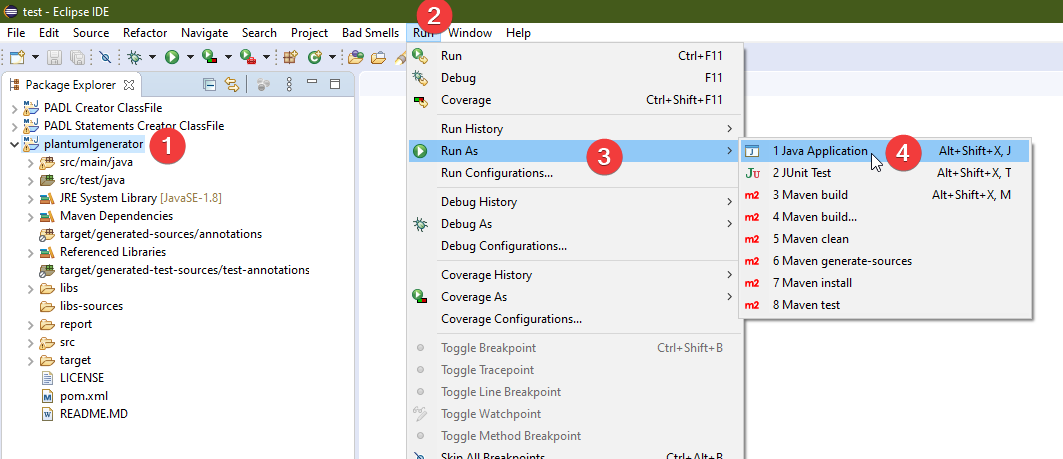
\includegraphics[scale=0.5]{images/run_as.png}\color{dimgray}
    \caption{\texttt{plantumlgenerator} run as Java Application}
\end{figure}

\begin{figure}[H]
    \centering
    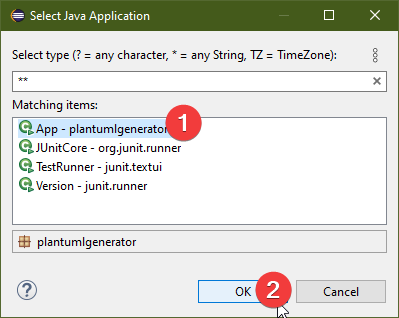
\includegraphics[scale=0.5]{images/main_app.png}\color{dimgray}
    \caption{Choose the target App}
\end{figure}

    \item \textbf{Step 3}: Copy and paste the path to the compiled .class files.\\
    An example to test is "./src/test/java/plantumlgenerator/padl/event/"\\
    Enter "n" to show the result in a new window (for copying the generated code).
    
\begin{figure}[H]
    \centering
    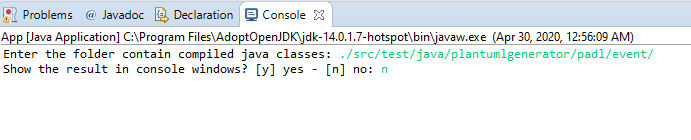
\includegraphics[scale=0.5]{images/console.png}\color{dimgray}
    \caption{enter the target folder containing compiled .class files}
\end{figure}

\begin{figure}[H]
    \centering
    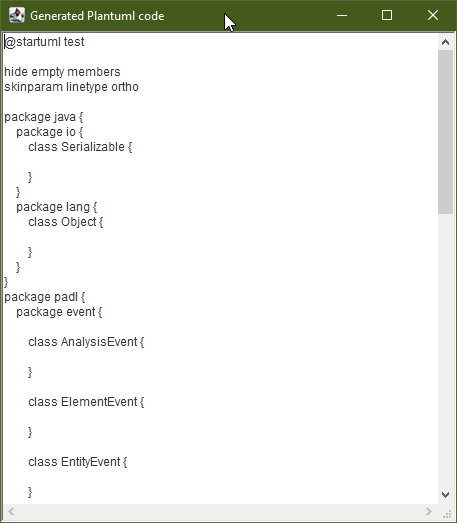
\includegraphics[scale=0.4]{images/result.png}\color{dimgray}
    \caption{Show the result in new window}
\end{figure}

    \item \textbf{Step 4}: [Optional] View the diagram online at \url{http://www.plantuml.com/plantuml/uml/}
    
\end{itemize}

The result diagram for \texttt{./src/test/java/plantumlgenerator/padl/event/} folder can be viewed \href{http://www.plantuml.com/plantuml/uml/ZL9BRi8m4DtFANm1E0DTe0gfLHTTT8Sq90CCiSUHFKHAA-vUegQMcBfIl60nxyFJUzbanQJNu9rILe0pj-Gez3gwGE50AKFkM7fC69nd8HrxSZ7fEGBqs7Hu8dV10TqNkFlxFN6S3lDhFERitYanUlx4WwSxMD0RbDyYzoYdFmPlXmirMfFUIfGUMs-Yq40ogOpRaw0VC-UjXM-MkVKKI7G1KPHrNC2R6Cyab51Z-eVAefIEs93RrHmhjDVOad_Xh9Fp4hhoiQwfXTwr97S1DwWSfHR9y6M87LbUTUs1C_yKOIm-q7UKwei3F2wuNk_dfW3AOXOe2vcxMMI2vZ-lOG-VCW3KgbojzcOH0B0TsXYbCtFVaBJNuBy1}{here}.

\begin{figure}[H]
    \centering
    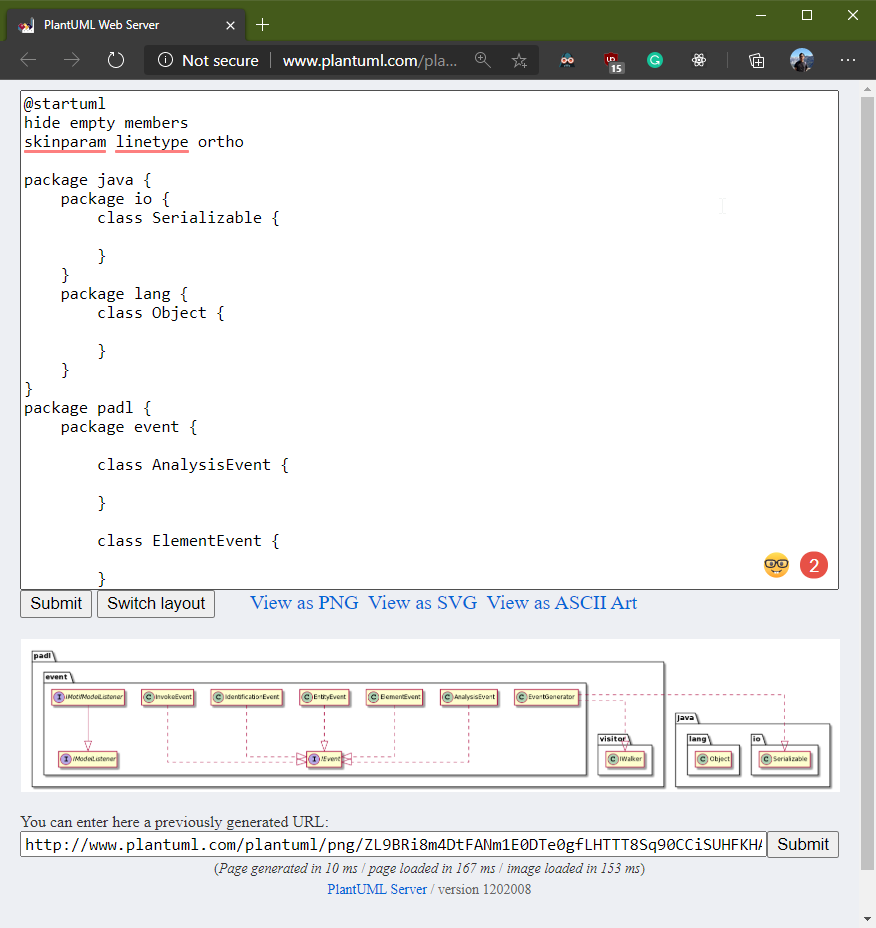
\includegraphics[scale=0.5]{images/diagram.png}\color{dimgray}
    \caption{The online diagram generator}
\end{figure}

\section{Test with other PADL meta-models}

In step 3 of section 3.2 above, if you paste another folder containing the compiled .class files, the tool will generate corresponding diagram for that folder.

One example with a much more complicated diagram is the diagram for the whole \texttt{padl} library at folder \texttt{./src/test/java/plantumlgenerator/padl/}. The result can be view online in svg format \href{http://www.plantuml.com/plantuml/svg/h9dXSY8t3CU_ynGyIXcutD0vGYQvv3wBNG4wlFQEB9ZGJjwzOVUgNXETaTFc0qFWzzVAiYt_T_aj2x0Skp0Lp3APxAd5ANQzdASTTXlaFCa7YZqmTDD04UNSupInxDDaqaDpW1rElyC9fdzEfgz_Vtz4QVnW-6i2v3nzG2O8z0Ti0hv-gT--JFHLvG7Yxbs0UKWHRVK_qAVd1dkX54lGUlCT6oaHzySerA4TpKZuA1JU9vowI-4aSUbIIq636LzVjCOzjE5DZV64KLIbyMOHmZbJ_gHVQz2tjGhOOHG768NaxE0kn6UCEY0BfIZ8MsXmkjI8PMoLMWnVACibiWSNsbxNQFrRZAy2Qk0oqTS7kOodT43bIgjYZw57VZz5DnGmFmg5V2t20JdYpojB9zzQcJyjFSPnEB_2NYpLKBG5DW7uclhzEztwNH_if6QRB0oDp2__EH9InRYcg9cdA40HURrzVPk5v8XHwa8jTQ7KgBxW2SDGdYfPXMAtOzo1UwfcEQU6_Bo_vlFKed-uskXI9dyoEdbIo-Tx72wL-EoNyh6Hn2vUbrZjXAYmkXYCu8ON68Qaucw5ia-jGwHztiNUGEEkxGrXQFtah6amPoVFUMmJuz7Z4eq7Jw3iAITf6tZRMuOL0zwsyhupBMD6lcImvXOPMs-dAeIy1JaoX73-_q9-JVsmoOVw4dh3Y23xq7tAufw3vHtJ2GI7bhFUPEGJR8AlHIzRIbrbmrfs_RWd_3klxjnO3UPPcwwJrw8v-RgSl1r3qOlJQVmLMlV8Vlfkj0irx0AtS0nI8z6AEWGC7GgoZsRgIEY45Vtf7iDGdhodtYLuy6-tXnuRylK-bGY8_rnup5ZEl-Z9pPvgaalRSVaq7y5_t9PcP8VGzWGsh0xD0skdA6EsD_FoSqRVVPbXOGgmPUOSyATdmPXhBx7Uwewh4MczAZJQptmwTPaEU3o5lQZjHXsgkdbaTCQtJ6XPeGxK2Qw03vxww5fmSTweXWUsmT40Up1rlmuuY2T9ooAN5PO_BlFYoaJFs39c-BIom31fPLxV-j6PRbaVhpcXGsMQm3BidKlJBvRXYl9ujxLb4ykAMpZHJgrz4TNR00_hRzNgEvsWcaudxvmJjPiErF2QHO5Xr0hqWtER6nQpo9l-qaODSrbwADg3xAs7gh55UnoA9Ev0x8VwPcBgM-kU_-l7q4AlnJKVoSsKgBxJhP7gvgyH_UiPUetm6uH3GV7B-PdlWMVCSBP-EJ7uYuNa26410dUS6ipvYc8yNR5T2fR3w_WlovYoK9EBx6sICNQHUXGArvRIYJ9fPlOXxdFnJvJ91OxJLKpyHopxwQln8m0hPw_zt-44EXJVOfnzNlqdoHEoK8FP9qLXQlBiTlKqdqDeZa6lwfHUbd30PvBpn_JBnSTqj-iF9lnjLIlyojG7b4NgWE8uNa6jTts81teDGLl2jX3ahqRDMBs960Z2_VykpZFGKgTF1HtGyVvyUEwM7UruIIVD_3vBYkwicqqkaTepE6_3iupdMtbU5hoI-lRsSLKimIgdPbIbr7MlZChIRPSygvK3gQJvU7mSbL70Qvbp6AfTJXtWSxMsDBmPsUZYKwVOW8cWlUhAjtV2u3S1AdN9dvv-4q1dzQVUNndDU3R1enLPhaMc_ea1wkqy3tNwJO3sHv7R1CWLCu7_-j22YpY6uJS1OZmnBhE2oTduN2XedzXNTGEJa_bzA1ManAyty-x1o5JIXpDqglLuicl05Mj8lJgk-dsjT6EEmvnd4rh4qNG9CB8A8OSwkNsTFSy80ys8Qm3ylpmMbaVnYAwfDkZbJzBV9d0SscKUeb7fKM5HI9fgHloL3UejO3xYXbbTQ3c6l2RSRfjv4sxtkFOXmhBdkwKsZDoXtAw2Oe42r7Ldts9tM2187LENZtfy8DQqOjhQTGKg991PNJWp0VakWhrKpyLDG5VWlUrnjS4tLRXiHbo3YWTaLnSi3SW3pymX0cV1vF78nnBiZjn95oSi3goA8gB_nFMUR3k9vEX_SlrUbFri0f3g9cAQ0Q5I4gbS6vaa5VVBcuE0hsCqzlrGETrBmc9reto4C7FA5M_PtCxLdjqvV6iKh3_lygSsQWR-WwZl79QjPlxkiLlpoOnxuGNLuSBoQ_DyO6ROIfjXDxTxhrP2RHXvgRcQGTqkwHIYd-wNRlriBOHL5tRCYmePZiixeSBQ19xDPXsZhwvFssVWavw-BsYQbbyz4_DHPfFsoMNVPvWO6CTbOMh3NVLoyNsA-RQk-eO_C8UPFjjF3o-E5HEqqhFSyU2RkXz4v5yQvRQ5TXw0unmjpdz-lOAN4JyM96HK1m83z9z58UCuKAzRsGVecRozxkViFP_c6MdxE567P5sGEM19kiT6ComNKDt4v7off-B5t1quSl0uqCg_vQhTzabjpoj91ataLBbQQsfXwR7iweB7lhveEH9s9cU_pkIGDuEUvcR0OridOZvhn1x4HZOdheF-yltNjzy_V_m1}{here}

\begin{figure}[H]
    \centering
    \includegraphics[scale=0.5]{images/padl_library_diagram.png}\color{dimgray}
    \caption{A view of the online class diagram of \texttt{padl} library}
\end{figure}

\end{document}
